\section{Discussion}
In this section, we further examine several additional properties and extensions of \method. We focus on the structural gap between likelihood-oriented estimation and generation quality, analyze how different conditioning and padding strategies affect block-causal \method in the first generation block, and present a preliminary exploration of VAE-based text compression for faster generation. Finally, we highlight the broader potential of \method for combining with other continuous modalities.

\definecolor{gentokenmatch}{RGB}{0,204,0}
\definecolor{gentokenmismatch}{RGB}{204,0,0}
\newcommand{\gttok}[1]{{\color{red!80!black}\bfseries\fontsize{11.5}{13.5}\selectfont #1}}
\newcommand{\genmatch}[1]{{\color{gentokenmatch}\textbf{#1}}}
\newcommand{\genmismatch}[1]{{\color{gentokenmismatch}\textbf{#1}}}

\subsection{The Structural Gap Between Likelihood-Oriented Estimation and Generation Quality}
\label{dis:ppl}

\begin{figure}[t]
    \centering
    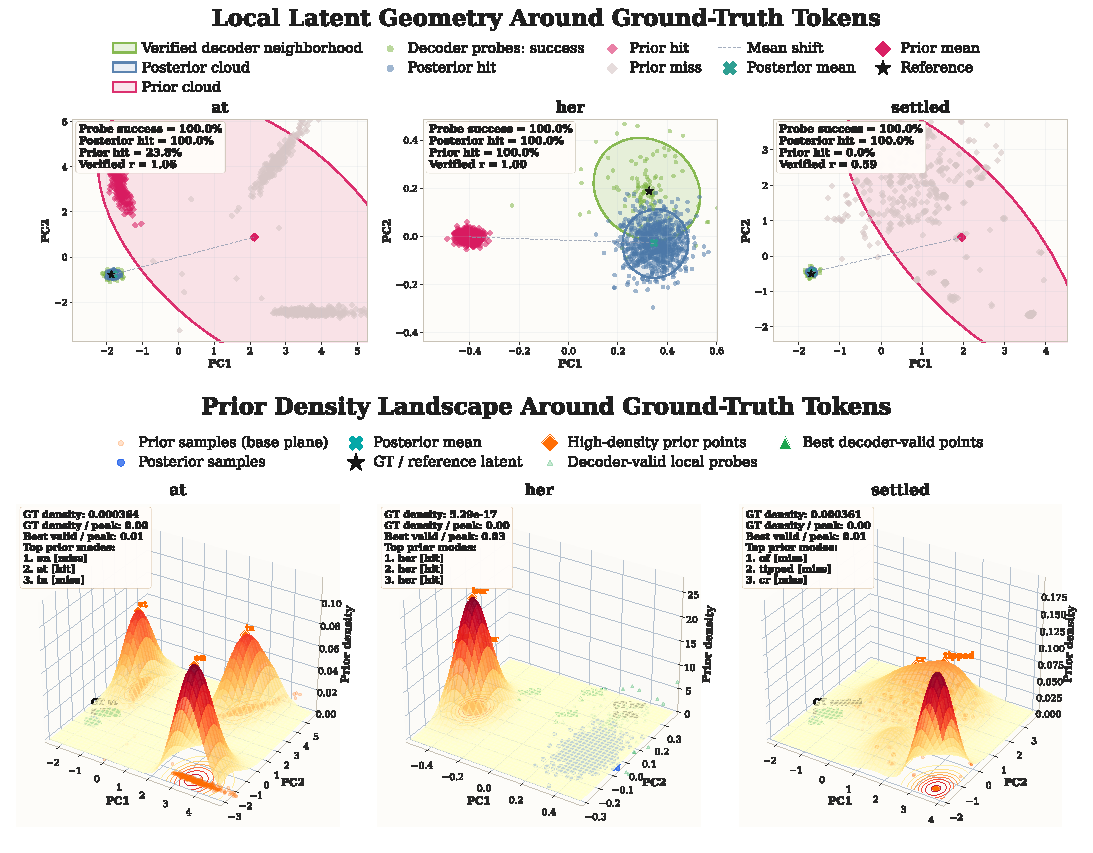
\includegraphics[width=\textwidth]{exp_fig/discussion/likelihood/exp_fig_discussion.pdf}
    \caption{\textbf{A local view of the mismatch between likelihood-oriented estimation and generation quality.} Top: local latent geometry around representative ground-truth tokens. Bottom: corresponding prior-density landscapes. High decoder probe success and posterior hit contrast with sharply varying prior hit and density alignment. Thus, good generation relies on covering decoder-valid regions, while likelihood estimation also demands precise local calibration around the gold posterior.}
    \label{fig:discussion_likelihood_geometry}
\end{figure}

This section studies a central phenomenon in continuous latent language models: generation quality can already be reasonable while likelihood-oriented PPL remains poor. The key reason is that these two metrics target different properties. Generation only requires the prior mass to reach semantically decoder-valid regions, whereas likelihood-oriented estimation additionally requires accurate local probability calibration around the posterior neighborhood of the ground-truth target.

Let
\[
x=(x^{\mathrm{pre}},x^{\mathrm{res}}),
\]
where $x^{\mathrm{pre}}$ is the prefix, $x^{\mathrm{res}}$ is the response, and $c$ denotes the conditional information induced by the prefix. The exact conditional marginal is
\begin{equation}
p(x^{\mathrm{res}}\mid c)
=
\int p_{\theta}(x^{\mathrm{res}}\mid z,c)\,p_{\psi}(z\mid c)\,\dd z,
\label{eq:resp_conditional_marginal_main_final}
\end{equation}
while the practically accessible quantity is the local score
\begin{equation}
\mathcal S_{\mathrm{resp}}(x)
=
\E_{q_{\phi}(z\mid x,c)}
\Big[
\log p_{\theta}(x^{\mathrm{res}}\mid z,c)
+\log p_{\psi}(z\mid c)
-\log q_{\phi}(z\mid x,c)
\Big].
\label{eq:resp_conditional_score_main_final}
\end{equation}
The mismatch between these two quantities is the starting point of our analysis.

\implicationbox{imp:main_gap_final}{
In continuous latent language models, good generation and good likelihood-oriented estimation are not equivalent. Generation depends on whether the prior reaches semantically valid latent regions, whereas likelihood-oriented estimation additionally depends on local density calibration around the gold posterior neighborhood.
}

This distinction is directly supported by Figure~\ref{fig:discussion_likelihood_geometry} and Table~\ref{tab:discussion_likelihood_example}. In Figure~\ref{fig:discussion_likelihood_geometry}, decoder probe success and posterior hit are consistently high, showing that the decoder can reliably recover the ground-truth token inside the posterior neighborhood. However, the prior hit rates vary sharply, indicating that the main issue is not decoder failure but prior misalignment around the gold latent region. Table~\ref{tab:discussion_likelihood_example} shows the same pattern at the token level: for \textbf{at}, the likelihood-derived PPL improves dramatically from $1.15\times10^6$ to $641.57$ and then $245.36$, while the generated token deteriorates from \textit{on} to \textit{in} and then to a comma. Similarly, for \textbf{her}, smaller likelihood-derived PPL under fixed VAE logSNR does not recover the correct token. Thus, lower likelihood-derived PPL does not necessarily imply better generation.

\begin{table}[t]
    \centering
    \footnotesize
    \setlength{\tabcolsep}{3.5pt}
    \renewcommand{\arraystretch}{1.12}

    \begin{tabularx}{\textwidth}{@{}X@{}}
        \toprule
        \textbf{Sample text.} At dawn the research vessel Meridian slipped out of the harbor and followed a chain of islands that looked like dark brushstrokes on the horizon. Mira stood \gttok{at} the bow with a notebook pressed against \gttok{her} jacket, listening as the engine \gttok{settled} into a steady hum and the crew argued about \ldots \\
        \bottomrule
    \end{tabularx}

    \vspace{0.55em}

    \begin{tabularx}{\textwidth}{@{}c c c c c c c c@{}}
        \toprule
        \makecell[c]{Ground-truth\\token}
        & \makecell[c]{Posterior\\$\log p(z \mid x)$}
        & \makecell[c]{Prior\\$\log p(z)$}
        & \makecell[c]{Decoder\\$\log p(x \mid z)$}
        & \makecell[c]{Likelihood-derived\\PPL $\downarrow$}
        & \makecell[c]{Generated\\token}
        & \makecell[c]{Gen. PPL $\downarrow$\\of \textbf{generated}}
        & \makecell[c]{Gen. PPL $\downarrow$\\of \textbf{ground-truth}} \\
        \midrule

        \multicolumn{8}{@{}l@{}}{\textbf{\textit{Direct training (unfixed VAE logSNR; measured effective VAE logSNR $\approx 4.5$)}}} \\
        \midrule
        \textbf{at} & 18.70 & 4.74 & $-3.62 \times 10^{-4}$ & $1.15 \times 10^{6}$ & \genmismatch{on} & \textbf{3.83} & 6.90 \\
        \textbf{her} & 22.61 & 2.26 & $-8.58 \times 10^{-6}$ & $6.93 \times 10^{8}$ & \genmatch{her} & \textbf{1.12} & 1.12 \\
        \textbf{settled} & 32.02 & 18.45 & $-8.54 \times 10^{-3}$ & $7.88 \times 10^{5}$ & \genmismatch{of} & \textbf{5.05} & $2.58 \times 10^{3}$ \\
        \midrule

        \multicolumn{8}{@{}l@{}}{\textbf{\textit{Fixed VAE logSNR = 1.0}}} \\
        \midrule
        \textbf{at} & -15.81 & -22.28 & $-2.10 \times 10^{-5}$ & \underline{641.57} & \genmismatch{in} & \underline{6.69} & 6.90 \\
        \textbf{her} & -11.79 & -15.68 & $-1.91 \times 10^{-5}$ & \textbf{48.98} & \genmismatch{the} & \underline{14.17} & 1.12 \\
        \textbf{settled} & -12.56 & -21.51 & $-1.40 \times 10^{-3}$ & \textbf{7740} & \genmismatch{of} & \textbf{5.05} & $2.58 \times 10^{3}$ \\
        \midrule

        \multicolumn{8}{@{}l@{}}{\textbf{\textit{Fixed VAE logSNR = 1.5}}} \\
        \midrule
        \textbf{at} & -8.04 & -13.54 & $-7.06 \times 10^{-5}$ & \textbf{245.36} & \genmismatch{,} & 90.94 & 6.90 \\
        \textbf{her} & -7.48 & -15.91 & $-4.96 \times 10^{-5}$ & \underline{$4.57 \times 10^{3}$} & \genmismatch{the} & \underline{14.17} & 1.12 \\
        \textbf{settled} & -6.12 & -15.71 & $-8.77 \times 10^{-5}$ & \underline{$1.46 \times 10^{4}$} & \genmismatch{went} & 460.16 & $2.58 \times 10^{3}$ \\
        \midrule

        \multicolumn{8}{@{}l@{}}{\textbf{\textit{Fixed VAE logSNR = 2.0}}} \\
        \midrule
        \textbf{at} & 11.50 & -6.41 & $-5.91 \times 10^{-5}$ & $5.99 \times 10^{7}$ & \genmismatch{behind} & 114.91 & 6.90 \\
        \textbf{her} & 13.74 & 0.21 & $-8.58 \times 10^{-5}$ & $7.53 \times 10^{5}$ & \genmismatch{it} & $3.07 \times 10^{3}$ & 1.12 \\
        \textbf{settled} & 10.30 & -6.57 & $-4.03 \times 10^{-3}$ & $2.14 \times 10^{7}$ & \genmismatch{came} & \underline{442.42} & $2.58 \times 10^{3}$ \\
        \bottomrule
    \end{tabularx}

    \caption{\textbf{Token-level comparison across direct training and fixed VAE logSNR settings.} Across the same target tokens, lower likelihood-derived PPL does not necessarily lead to better generation. This token-level evidence further illustrates the structural gap between likelihood-oriented estimation and generation quality.}
    \label{tab:discussion_likelihood_example}
\end{table}

\implicationbox{imp:semantic_vs_prob_smoothing_final}{
In \method, generation quality is more related to semantic smoothness of the latent space, whereas likelihood-oriented PPL is more sensitive to probability-space smoothness shaped by the VAE logSNR. Since these two forms of smoothness are different, generation and PPL need not be aligned.
}

The fixed VAE logSNR settings in Table~\ref{tab:discussion_likelihood_example} should therefore be interpreted as changing the smoothness of the latent probability space rather than merely tuning a hyperparameter. Lower VAE logSNR corresponds to a flatter local density landscape, which tends to reduce pointwise density mismatch and improve likelihood-derived PPL. However, such smoothing can also blur local semantic structure and bias the model toward generic but semantically suboptimal continuations, such as \textit{in}, \textit{the}, or \textit{went}. By contrast, direct training yields much worse likelihood-derived PPL, but sometimes preserves more appropriate semantic behavior, such as correctly generating \textbf{her}.

\obsbox{
\textbf{Summary.}
In \method, generation quality primarily reflects the semantic smoothness of the latent space, whereas likelihood-oriented PPL is more sensitive to the smoothness of the latent probability space shaped by the VAE logSNR. As a result, better generation does not necessarily imply better PPL, and vice versa.
}

\begin{figure}[t]
    \centering
    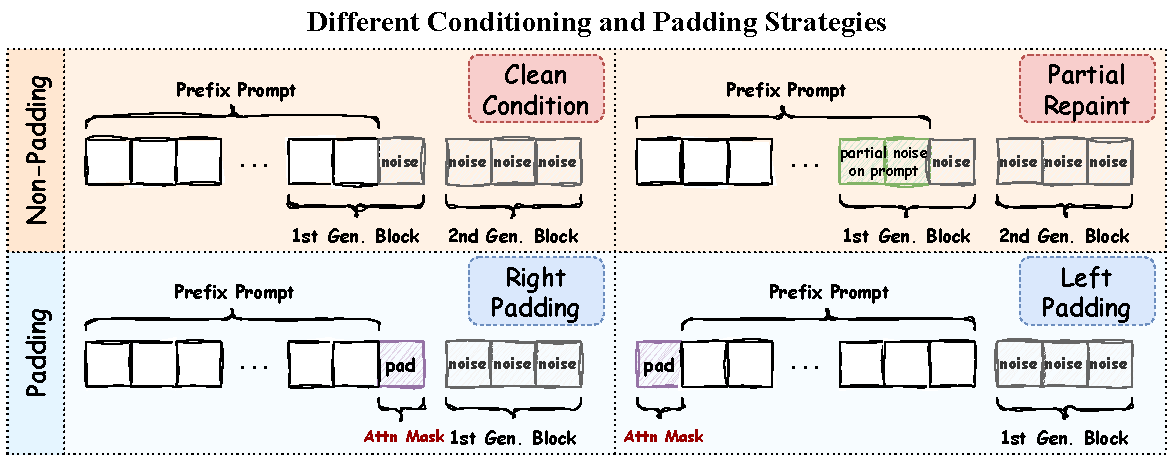
\includegraphics[width=1\textwidth]{exp_fig/discussion/cond_pad/condition_strategies.pdf}
    \caption{\textbf{Different conditioning and padding strategies in the first generation block.} The first generation block is a mixed region that contains both known prompt latents and unknown latents to be generated. Clean condition repaint keeps the known region fixed as a stable condition throughout denoising, partial repaint injects timestep-matched noisy guidance only during part of the trajectory, and left/right padding instead modify the layout of the known region without explicit repaint correction.}
    \label{fig:cond_strategies}
\end{figure}

\begin{table}[t]
    \centering
    \caption{\textbf{Impact of first-block conditioning strategies.} Clean condition repaint performs best, indicating strong, persistent conditioning is optimal for the first block's mixed denoising. Conversely, partial repaint is much weaker, reducing $m$ degrades performance, and increasing $t$ yields no stable gains. Left and right padding outperform partial repaint but remain inferior to clean conditioning.}
    \label{tab:first_block_conditioning}
    \small
    \setlength{\tabcolsep}{3.8pt}
    \renewcommand{\arraystretch}{1.10}
    \begin{tabular*}{\linewidth}{@{\extracolsep{\fill}}lccccccccc}
        \toprule
        \multirow{2}{*}{\textbf{Task}}
        & \multicolumn{3}{c}{\textbf{Partial repaint ($t=1$)}}
        & \multicolumn{3}{c}{\textbf{Partial repaint ($t=3$)}}
        & \multirow{2}{*}{\textbf{Clean cond.}}
        & \multirow{2}{*}{\textbf{Left pad.}}
        & \multirow{2}{*}{\textbf{Right pad.}} \\
        \cmidrule(lr){2-4} \cmidrule(lr){5-7}
        & \textbf{$m=1.0$} & \textbf{$m=0.7$} & \textbf{$m=0.3$}
        & \textbf{$m=1.0$} & \textbf{$m=0.7$} & \textbf{$m=0.3$}
        & \multicolumn{3}{c}{} \\
        \midrule
        \textbf{Lambada} & 8.5 & 8.5 & 6.6 & 7.0 & 7.3 & 5.6 & \textbf{37.1} & 24.6 & \underline{24.7} \\
        \textbf{MMLU}    & 7.9 & 7.9 & 7.8 & 7.6 & 6.7 & 7.0 & \textbf{11.9} & 8.4  & \underline{11.5} \\
        \textbf{SIQA}    & 8.8 & 8.7 & 8.2 & 13.3 & 13.0 & 12.0 & \textbf{24.8} & \underline{14.9} & 13.8 \\
        \midrule
        \textbf{Avg.}    & 8.4 & 8.4 & 7.5 & 9.3 & 9.0 & 8.2 & \textbf{24.6} & 16.0 & \underline{16.7} \\
        \bottomrule
    \end{tabular*}
\end{table}

\subsection{Impact of Conditioning and Padding Strategies in the First Generation Block}
\label{sec:first_block_conditioning}

In the first generation block, the input contains both known prompt latents and unknown latents to be generated. Figure~\ref{fig:cond_strategies} illustrates four representative strategies for handling this mixed region. Partial repaint injects timestep-matched noisy guidance on the known region, where $t$ controls the number of repaint repetitions and $m$ controls the fraction of the denoising trajectory that receives such guidance. Clean condition repaint instead keeps the known region fixed as clean guidance throughout denoising. By contrast, left and right padding do not explicitly repaint the known region, but only change its positional layout relative to the generated region. Notably, under the random-length setting, all aforementioned conditioning modes maintain strict consistency between training and inference.

As shown in Table~\ref{tab:first_block_conditioning}, clean condition repaint consistently achieves the best performance across all tasks. In contrast, partial repaint is substantially weaker, and reducing $m$ generally further degrades performance, indicating that shortening the guided portion makes the known region harder to preserve. Increasing the repaint repetitions from $t=1$ to $t=3$ also does not bring stable gains, suggesting that repeated early corrections cannot compensate for weak conditioning. Left and right padding are often stronger than most partial repaint settings because they avoid explicitly re-noising the known region, but still remain clearly below clean condition repaint. This suggests that positional layout alone is insufficient: padding does not provide a stable condition throughout denoising, and may further complicate the block-causal attention pattern.

Overall, these results show that the key challenge of the first generation block is to preserve the prompt-conditioned region while generating the remaining unknown part. For this mixed denoising problem, strong and persistent conditioning is more effective than partial noisy correction or positional layout alone. More details are provided in Appendix~\ref{app:first_block_conditioning_detail}.

\subsection{Compression of the Latent Space}
\label{dis:latent_compression}

\begin{table}[t]
    \centering
    \caption{\textbf{Performance under different sample labels and VAE patch sizes.} Patch size 2 is overall weaker, but this gap stems mainly from the Prompt Len Mod1 case (indivisible lengths). On Prompt Len Mod0, patch size 2 becomes competitive and even outperforms size 1. This suggests the weakness arises from boundary misalignment rather than latent compression itself.}
    \label{tab:sample_label_vae_patch}
    \small
    \setlength{\tabcolsep}{5pt}
    \renewcommand{\arraystretch}{1.10}
    \begin{tabular*}{\textwidth}{@{\extracolsep{\fill}}lcccccc}
        \toprule
        \textbf{Sample Label}
        & \multicolumn{2}{c}{\textbf{Overall}}
        & \multicolumn{2}{c}{\textbf{Prompt Len Mod0}}
        & \multicolumn{2}{c}{\textbf{Prompt Len Mod1}} \\
        \cmidrule(r){1-1} \cmidrule(lr){2-3} \cmidrule(lr){4-5} \cmidrule(l){6-7}
        \textbf{VAE Patch Size}
        & \textbf{p1} & \textbf{p2}
        & \textbf{p1} & \textbf{p2}
        & \textbf{p1} & \textbf{p2} \\
        \midrule
        \textbf{Lambada} & \textbf{31.10} & 17.40 & 32.11 & \textbf{34.55} & \textbf{30.12} & 0.79 \\
        \textbf{MMLU}    & \textbf{5.40}  & 3.90  & 6.89  & \textbf{7.68}  & \textbf{3.86}  & 0.00 \\
        \textbf{SIQA}    & \textbf{11.10} & 6.10  & \textbf{12.92} & 12.13 & \textbf{9.26} & 0.00 \\
        \midrule
        \textbf{Avg.}    & \textbf{15.87} & 9.13  & 17.31 & \textbf{18.12} & \textbf{14.41} & 0.26 \\
        \bottomrule
    \end{tabular*}
\end{table}

This section discusses whether compressing the text sequence in the VAE is beneficial for \method. We train two Text VAEs with the same latent dimensionality ($d=128$) but different patch sizes: $p1$ maps each token to one latent, while $p2$ compresses every two tokens into one latent. All other settings follow Section~\ref{exp:rq4}: the DiT block size is $16$, the training noise schedule uses logit-normal sampling with $\mathrm{loc}=1$ and $\mathrm{scale}=0$, and inference uses $16$ denoising steps with CFG $=7.0$. In Table~\ref{tab:sample_label_vae_patch}, \textit{Overall} reports the full evaluation result, while \textit{Prompt Len Mod0} and \textit{Prompt Len Mod1} group samples by whether the prompt length is divisible by $2$.

\implicationbox{imp:latent_compression_main}{
The weakness of patch size $2$ does not mainly come from compression itself, but from the boundary case where the prompt length is not divisible by the patch size. Once the latent grouping is well aligned with the text sequence, compression can instead become beneficial.
}

At the overall level, $p2$ is much worse than $p1$. However, the parity split shows that this gap is almost entirely caused by \textit{Prompt Len Mod1}. For odd-length prompts, $p2$ nearly collapses on all tasks, whereas on \textit{Prompt Len Mod0}, namely the even-length case seen by the patching rule, $p2$ becomes competitive and even slightly surpasses $p1$ on average. This suggests that the current failure is not evidence against latent compression itself, but against a compression scheme that does not robustly handle non-divisible sequence boundaries.

The reason is likely that, under patch size $2$, odd-length prompts necessarily involve padding or incomplete token groups during compression. If this boundary pattern is not properly learned, the compressed prompt latent becomes semantically shifted. In \method, this issue is particularly severe because the prompt latent is the clean condition for subsequent block-wise prior generation rather than a weak auxiliary representation. Once the prompt-side latent is biased, the error propagates through denoising and finally harms conditional decoding, which naturally explains the near-zero performance on \textit{Mod1}.

By contrast, the \textit{Mod0} result is encouraging. It shows that when the latent grouping is semantically valid, compressing two tokens into one latent does not necessarily hurt generation and may even help it. This is consistent with the core idea of \method: the latent space is not intended to preserve a token-aligned recovery path, but to provide a lower-rate representation for global semantic organization, while the decoder handles local realization. Under this view, moderate compression can be beneficial because each latent summarizes a larger textual span and thus better matches the role of the prior.

This also makes latent compression attractive from the efficiency perspective. Under the same DiT block size, one denoising block corresponds to $\text{patch size} \times \text{block size}$ text tokens after decoding. Therefore, with block size $16$, patch size $1$ covers $16$ text tokens per block, while patch size $2$ covers $32$. If the boundary issue can be resolved, larger patch sizes may improve both semantic abstraction and generation efficiency.

\obsbox{
\textbf{Summary.}
Table~\ref{tab:sample_label_vae_patch} suggests that latent compression is a promising direction for \method. Its current limitation mainly comes from unstable handling of non-divisible sequence boundaries, while the aligned even-length case already shows that compressed latents can support both stronger semantic abstraction and faster generation.
}

\subsection{Robustness of VAE Latent Reconstruction}
\label{dis:vae_recon_robustness}

\begin{wrapfigure}{r}{0.52\textwidth}
    \centering
    \vspace{-0.5em}
    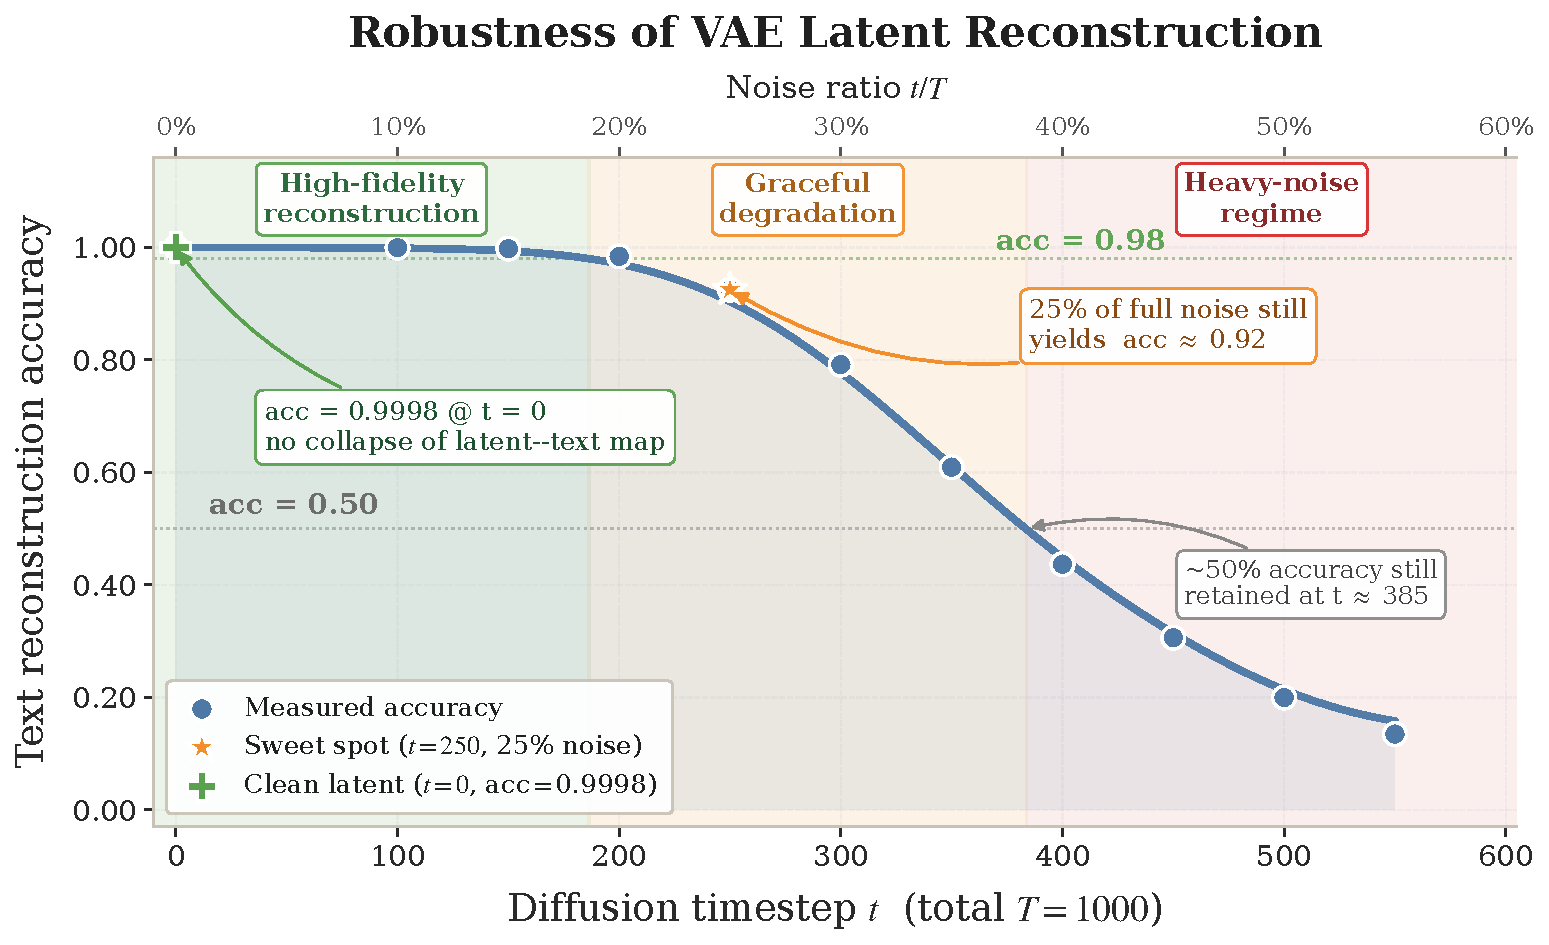
\includegraphics[width=0.50\textwidth]{exp_fig/discussion/robust/vae_noise_robustness.pdf}
    \vspace{-0.8em}
    \caption{\textbf{Robustness of VAE latent reconstruction.} The VAE preserves near-perfect reconstruction at low noise and degrades gracefully under stronger perturbations, indicating a stable latent--text mapping.}
    \label{fig:vae_recon_robustness}
    \vspace{-1.0em}
\end{wrapfigure}

We further analyze the robustness of the VAE latent space from the reconstruction perspective. As shown in Figure~\ref{fig:vae_recon_robustness}, the VAE achieves nearly perfect reconstruction at $t=0$, indicating that the learned latent--text mapping remains highly faithful and does not collapse. Moreover, the reconstruction accuracy stays very high throughout the low-noise regime, and still remains around $0.92$ at $t=250$, before degrading more noticeably under heavier noise.

These results suggest that the latent space learned by the VAE is not merely a fragile compressed code, but a stable and broadly usable intermediate representation for text. In particular, the graceful degradation pattern indicates that semantic information is not destroyed abruptly by small or moderate perturbations, which further supports the view that the VAE latent space in \method is sufficiently robust to serve as the semantic interface for subsequent prior modeling.

\subsection{Towards a Unified Approach with Image Modalities}

\begin{figure}[tp]
    \centering
    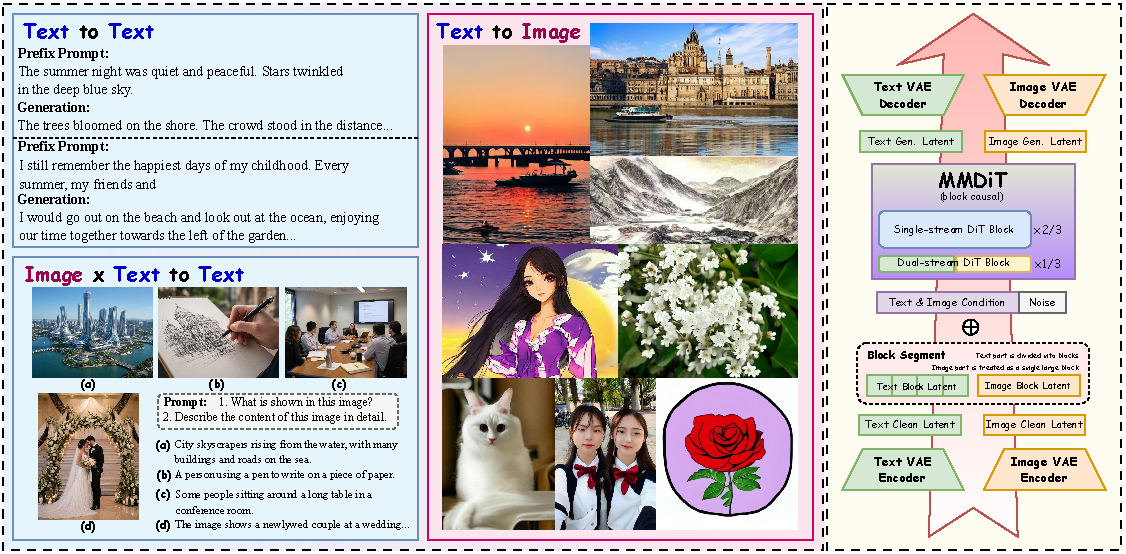
\includegraphics[width=\textwidth]{exp_fig/discussion/unified/unified_samples.pdf}
    \caption{\textbf{Preliminary qualitative examples of unified text-image modeling.}
    Left: text-only continuation and image-conditioned text generation. Middle: text-to-image results with only pretraining. Right: a schematic extension of \method, where text and image are mapped into modality-specific continuous latents and modeled by a shared block-causal prior.}
    \label{fig:unified_samples}
\end{figure}

A broader implication of \method is that it provides a natural bridge from discrete text to continuous multimodal modeling. The key idea of unified modeling is not merely to place text and image into one backbone, but to map heterogeneous observations into a shared continuous latent interaction space, where higher-level semantics can be organized under common dynamics.

A natural extension of \method follows the same probabilistic decomposition as in the text-only setting. Let $x^{\text{text}}$ and $x^{\text{img}}$ denote the text and image observations, and let their modality-specific latent variables be
\[
z^{\text{text}}_0 \sim q_{\phi_{\text{text}}}(z \mid x^{\text{text}}), 
\qquad
z^{\text{img}}_0 \sim q_{\phi_{\text{img}}}(z \mid x^{\text{img}}).
\]
We then define a joint latent state
\[
\tilde z_0 = \bigl(z^{\text{text}}_0, z^{\text{img}}_0\bigr),
\]
and model the unified generative process as
\[
p(x^{\text{text}}, x^{\text{img}}, \tilde z_0)
=
p_{\theta}\!\left(x^{\text{text}}, x^{\text{img}} \mid \tilde z_0\right)
\, p_{\psi}(\tilde z_0).
\]
Under this view, modality-specific VAE encoders and decoders are responsible for surface-level representation and realization, while the shared prior models the higher-level semantic structure and cross-modal dependency in latent space.

This perspective is consistent with the central modeling principle of \method. In Cola DLM, diffusion is not used for token-level observation recovery, but for latent prior transport:
\[
z_1 \sim p_1, 
\qquad
z_0 = \Phi^{\psi}_{0\leftarrow1}(z_1),
\qquad
x \sim p_{\theta}(x \mid z_0).
\]
In the unified setting, the same idea extends to the multimodal latent state $\tilde z_0$: the shared block-causal MMDiT prior transports and organizes the joint latent semantics, while the modality-specific decoders handle the final text or image realization. Therefore, continuity is introduced at the level of prior modeling rather than direct token or pixel recovery.

From the ELBO viewpoint, the benefit of such a decomposition is also conceptually clear. A unified latent-variable objective takes the form
\[
\mathbb{E}[\mathcal{L}_{\mathrm{ELBO}}]
=
\mathbb{E}_{q}\!\left[\log p_{\theta}(x^{\text{text}}, x^{\text{img}} \mid \tilde z_0)\right]
- I\!\left((X^{\text{text}}, X^{\text{img}});\tilde Z_0\right)
- \mathrm{KL}\!\left(\bar q(\tilde z_0)\,\|\,p_{\psi}(\tilde z_0)\right),
\]
which shows the same division of labor as in the text-only case: the latent variable carries compressed global semantics, while the decoder is responsible for modality-specific realization. In this sense, unified modeling is not simply parameter sharing across modalities, but a shared semantic prior over heterogeneous observations.

Figure~\ref{fig:unified_samples} presents a preliminary prototype of this idea. In the current design, the text sequence is divided into blocks, while the image latent is treated as a single large block. Specifically, the image representation is obtained via an Image VAE trained on internal multi-resolution data (256 / 384 / 640 / 1024), with a spatial downsampling factor of 16 and 64 latent channels, providing a compact yet expressive latent space for visual content. The shared block-causal MMDiT prior operates over both text blocks and image latents, supporting intra-modal processing as well as cross-modal interaction. Within a unified framework, this enables text-to-text continuation, image-conditioned text generation, and text-to-image generation. We jointly optimize these tasks on internal image–text pairs during training. For the text-to-image task, we first train on 256-resolution data for 80k steps with a global batch size of approximately 3k, and then continue training on 640-resolution data for 10k steps with a global batch size of approximately 1k. For image-conditioned text generation, we adopt the same batch size configuration and train for approximately 50k steps. More result samples are provided at~\ref{app:unified_results}.

These results should be interpreted primarily as qualitative evidence of feasibility. As the current prototype remains at an early stage of training, and our experiments are limited to moderate pretraining on in-house 256 and 640 resolution data, without extensive high-quality data curation or supervised fine-tuning. The goal of this section is not to present a mature multimodal system. Rather, it is to demonstrate that the hierarchical latent-prior formulation of \method naturally extends beyond text-only generation. In future work, we plan to conduct more comprehensive unified multimodal training. More broadly, these findings suggest that decoupling global latent organization from modality-specific realization may offer a structurally clean and scalable path toward more native unified generative models.

\obsbox{
\textbf{Summary.}
These preliminary results suggest that \method naturally extends to unified text--image modeling. A shared block-causal prior organizes global and cross-modal semantics, while modality-specific decoders handle final realization. Although still early-stage and qualitative, this prototype already shows a promising bridge from language generation to native multimodal generative modeling.
}